In coverage based evolutionary fuzz testing, every input that triggers new behavior will be added to an interesting seed queue which will then be used as the template file for next mutation. While as the testing goes on, more and more new seed files will be added into the queue, especially for large-scale software, the size of the queue can quickly reach a very large number. Obviously, mutating for every test case in the queue will last for a long time, so, in order to find more bugs or maximize the coverage in a budget time, we should introduce search strategy to prioritize the test cases. 

Figure~\ref{motivate-example} describes the motivation of the seed search strategy for prioritizing the test cases. Suppose the state space of a program is modeled as a two-dimensional space, and each input will be mapped to a point in the space. Fuzz testing always starts from an initial seed test case (the red point in the figure). The test cases that generated from this red point will cover some new paths in the state space (shown as the black points plus with A and B). Then, in evolutionary fuzz testing, a test case will be picked up from such new paths as the seed file for next round of mutation. 

Consider seed \textit{A} and \textit{B} in this figure, the \emph{distance} from the initial seed file to \textit{A} is much shorter than \textit{B}, which, in other words, means that \textit{A} is more \textbf{\textit{similar}} with the initial seed file than \textit{B}. So if \textit{A} is selected as the next seed file to mutate, then there will be only two new paths to be touched as most of the coverage area of seed \textit{A} is overlapped with what of the initial seed file. As seed \textit{B} has a longer distance to the initial seed file than seed \textit{A} and the new coverage area of \textit{B} have less overlap with that of the initial seed file, so if seed \textit{B} is selected as the next seed, we can quickly cover more paths than selecting seed \textit{A}.

Based on this insight, we proposed a test case prioritization method based on similarity. Our method leverages some distance measures in regression testing, i.e. \textit{Euclidean distance}, \textit{Cosine similarity} and \textit{Jaccard index}, as the classification metrics for test case prioritization. All the test cases that trigger new behaviors will be mapped into vectors, and then our method assigns a weight for each test case based on the distance measures to other test cases. At last, the fuzzer will select a global optimum seed file according to the weight value as the next seed file.

In the following sections, we firstly introduce these three similarity measures and then explain how a test case is mapped as a numerical vector. The seed searcher selection algorithm is then described as well as the distance calculation of the test case vectors.

\begin{figure}
\centering
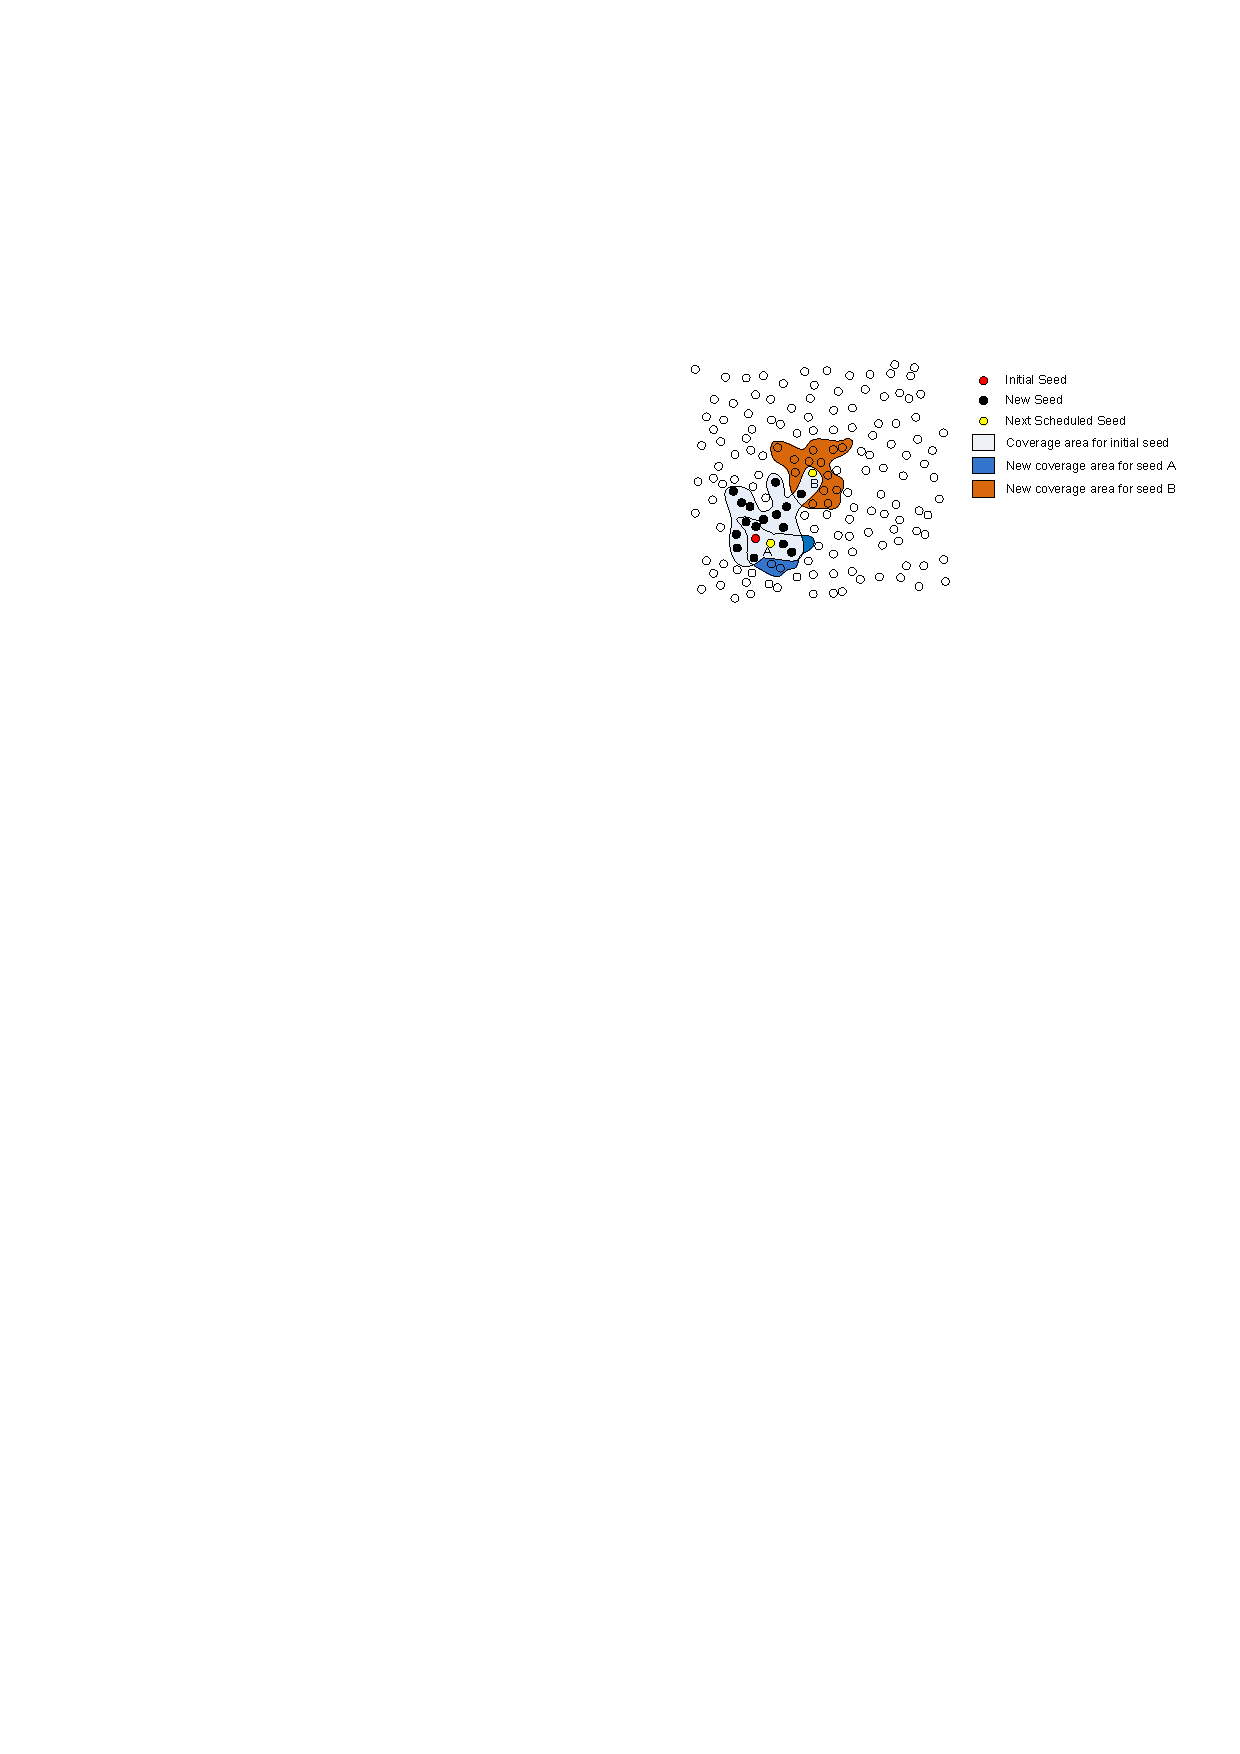
\includegraphics[width=0.7\textwidth]{figures/motivate-example.pdf} 
\caption{An motivate example.}\label{motivate-example}
\end{figure}


\subsection{Distance Metrics}
For two vectors $\mathbf{X} = (x_1, x_2, \cdots, x_N)$ and $\mathbf{Y} = (y_1, y_2, \cdots, y_N)$, the corresponding similarity metrics for \textit{Euclidean Distance}, \textit{Cosine Similarity} and \textit{Jaccard Index} are listed as follows.

\begin{enumerate}
\item Euclidean Distance (EU)

The Euclidean Distance between two vectors is defined as follows:
\begin{center}
$EU(\mathbf{X}, \mathbf{Y}) = \displaystyle \sqrt{\sum_{i=1}^{N} (x_i-y_i)^2}$
\end{center}


\item Cosine Similarity (CS)

The consine similarity between $\mathbf{X}$ and $\mathbf{Y}$ is defined as follows:

\begin{center}
$CS(\mathbf{X}, \mathbf{Y}) = \displaystyle \sqrt{\frac{\mathbf{X}^T \cdot \mathbf{Y}} {\| \mathbf{X} \|\| \mathbf{Y} \|}}$
\end{center}
where $\mathbf{X}^T$ is a transposition of vector $\mathbf{X}$ and $\| \mathbf{X}\|$ is the Euclidean Distance of
vector $\mathbf{X}$. Similarly, $\|\mathbf{Y}\|$ is the Euclidean norm of vector $\mathbf{Y}$. In essence, \textit{CS} is the cosine of the angle between $\mathbb{X}$ and $\mathbf{Y}$ in the N-dimensional space. For Cosine similarly, the corresponding distance is defined as:

\begin{center}
$D(\mathbf{X},\mathbf{Y}) = 1 - CS(\mathbf{X},\mathbf{Y})$
\end{center}

\item Jaccard Index (JI)

The Jaccard Index between $\mathbf{X}$ and $\mathbf{Y}$ is defined as follows:

\begin{center}
$JI(\mathbf{X}, \mathbf{Y}) = \displaystyle \frac{\mathbf{X} \cdot \mathbf{Y}}{\mathbf{X} \cdot \mathbf{Y}+\omega(\|\mathbf{X}\|^2+\|\mathbf{Y}\|^2-2(\mathbf{X} \cdot \mathbf{Y}))}$
\end{center}

where $\mathbf{X} \cdot \mathbf{Y}$ is the inner product of $\mathbf{X}$ and $\mathbf{Y}$. 
When $\omega$ is equal to 1, the above formula is called Jaccard Index and its corresponding distance is defined as follows:

\begin{center}
$D(\mathbf{X},\mathbf{Y}) = 1 - JI(\mathbf{X},\mathbf{Y})$
\end{center}

\end{enumerate}

\subsection{Mapping test case to vector space}
In order to measure the distances between test cases, all the test cases should be mapped into vector space. The Mapping could be performed both from input space and state space. However, mapping from input space cannot reflect the real relationship between test cases when considering the code coverage. As shown in Figure~\ref{distance-illusion}, multiple inputs can steer the program to execute the same path. Specifically, considering the three test cases namely \texttt{A.jpeg}, \texttt{B.jpeg} and \texttt{C.jpeg} in this figure, suppose the corresponding contents are shown as follows:

\texttt{A.jpeg}: \texttt{$\backslash$xFF$\backslash$xD8$\backslash$xAA$\backslash$xBB$\backslash$xCC$\backslash$xDD}

\texttt{B.jpeg}: \texttt{$\backslash$xFF$\backslash$xD8$\backslash$xDD$\backslash$xCC$\backslash$xBB$\backslash$xAA}

\texttt{C.jpeg}: \texttt{$\backslash$xFE$\backslash$xD8$\backslash$xAA$\backslash$xBB$\backslash$xCC$\backslash$xDD}

Obviously, if we calculate the Euclidean Distance between these three files based on the contents, EDAB will be larger than $ED_{AC}$ as there are more bytes have been modified, which means \texttt{A.jpeg} and \texttt{C.jpeg} are more similar (as shown in Figure~\ref{distance-illusion}). However, for most of the JPEG process programs, \texttt{A.jpeg} and \texttt{B.jpeg} will execute the same path and \texttt{C.jpeg} will execute another path as \texttt{C.jpeg} is not a proper JPEG file (bad magic number). So from the viewpoint of program, file \texttt{A.jpeg} and \texttt{B.jpeg} are more similar than \texttt{A.jpeg} and \texttt{C.jpeg} even though \texttt{A.jpeg} and \texttt{C.jpeg} have only one bit difference. Because the objective is to maximize the coverage of the program, so all the test cases should be mapped into vectors in state space and then calculating the distance.

In \cite{R1} all test cases are represented by the branches covered as a branch coverage vector \textbf{\textit{V}} = $(v_1, v_2, \cdots, v_N)$, where $v_i$ is 0 means the branch is covered, otherwise 1. However, different test cases can affect different branches, so the mapped vectors may have different lengths which cannot be used directly for distance calculation. Meanwhile, it will be very difficult to construct such vectors because it is hard to obtain all the branches and list them orderly in each vector to avoid obfuscation between vectors. AFL utilizes a fixed size bitmap to record the executed path information of a test case. And what’s more, AFL depends on analyzing this bitmap to determine whether a test case triggers new behavior, which means this bitmap contains enough information to reflect the characteristics of the test case from the viewpoint of a program. So we select the bitmap used in AFL our mapped vector to mitigate the costly mapping as the list of ordered branches.

\begin{figure}
\centering
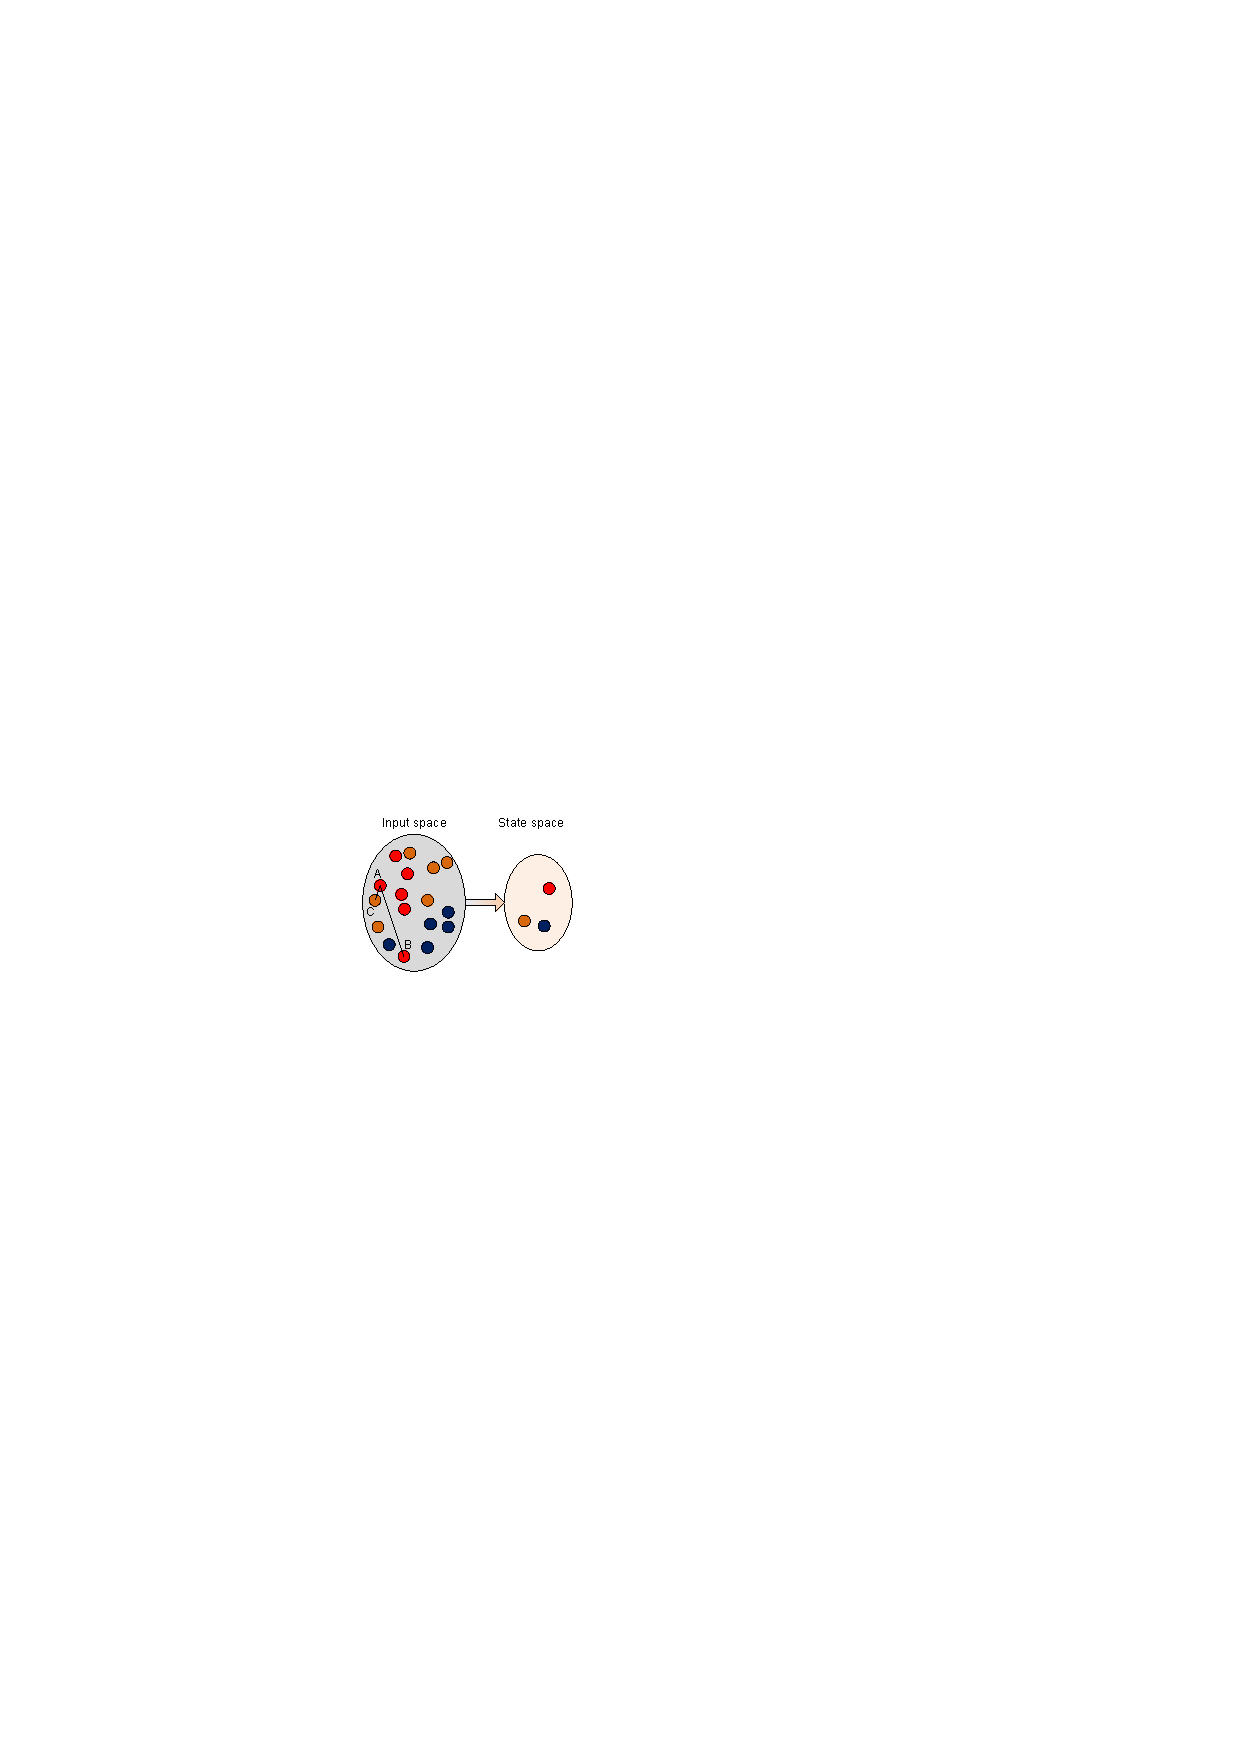
\includegraphics[width=0.5\textwidth]{figures/distance-illusion.pdf} 
\caption{An illusion for distance.}\label{distance-illusion}
\end{figure}

\subsection{Searching Method}
Based on the mapped bitmap vectors, the test case queue in the fuzzer is enhanced by assigning each test case with weight $W$ which is obtained from the distance between every two test cases. Whenever a new seed file is found, the distance between this seed file and all the other files in the queue will be measured to calculate $W$. And meanwhile, the weight of all the other files in the queue will be updated according to the distance to the new seed file. 


Rather than selecting the seed file that has the longest distance to the current seed file which is only a \emph{local optimum solution}, our search method selects the file that takes the longest average distance from all the other test cases as the next seed file. By doing this, we can achieve the \emph{global optimum solution} for this searching problem. The weight $W$ for $t_k$ is defined as follows:

\begin{center}
$W_k = \displaystyle\frac{1}{N} \sum_{i=0}^{N} D(t_i, t_k)$
\end{center}

where $D(t_i, t_k)$ denotes the distance between $t_i$ and $t_k$ based on the three distance measures mentioned before, and $N$ is the size of the test case queue. 